Le chapitre I de ce rapport est consacré à la présentation de l’organisme d’accueil, une étape cruciale pour comprendre le cadre dans lequel le stage s’est déroulé. Cette section commence par une introduction à l'université puis à l’entreprise et à l’équipe , détaillant l'historique, la mission, ainsi que les produits et services principaux de l'entreprise. Elle continue par une description de l’équipe, incluant la composition et les rôles des membres, ainsi que les objectifs et missions de l’équipe. Enfin, la structure organisationnelle est examinée, mettant en lumière la position de l’équipe au sein de l’entreprise. Le chapitre se conclut par la définition des objectifs du stage, détaillant les objectifs globaux, l'importance et l’impact attendu sur l’entreprise, les compétences à développer, ainsi que les livrables et les indicateurs de réussite.
\section{Présentation de l’UPEC}

L'Université Paris-Est Créteil ou \textbf{UPEC} est une université publique fondée en 1970. Située en Île-de-France, elle est l'une des principales institutions académiques de la région. L'\textbf{UPEC} est réputée pour son engagement à fournir une éducation de qualité et à promouvoir la recherche scientifique. Elle offre une variété de formations en sciences humaines et sociales, médecine, sciences économiques et gestion, sciences et technologies, ainsi qu'en droit et sciences politiques.
Je suis actuellement en troisième année de licence informatique à l'\textbf{UPEC}, où j'acquiers des compétences en programmation, développement de logiciels et gestion de systèmes informatiques.

\begin{figure}[H]
	\begin{center}
		\fbox{
\includegraphics[scale=0.5]{images/upecred.png}}
		\caption{UPEC}
	\end{center}
\end{figure}

\section{Présentation d’ Exakis Nelite}
\subsection{Présentation de l'entreprise}

Exakis Nelite, une entreprise de conseil en transformation digitale fondée en 2001, est devenue une entité clé du groupe Magellan Partners depuis 2008. Sa mission est d’accompagner les entreprises dans l’adoption et l’intégration des solutions Microsoft, offrant des services de conseil, d’intégration, de développement et de support. Exakis Nelite s’engage à fournir des solutions innovantes et adaptées, participant activement à la transformation numérique de ses clients grâce à une expertise technique de haut niveau. L'entreprise est spécialisée dans plusieurs domaines clés de la transformation digitale portés par les équipes :
\begin{itemize}
    \item[•] \textbf{Modern Work} : Elle déploie des solutions collaboratives et de productivité comme Microsoft365, met en place des intranets et des applications métiers, et accompagne au changement pour maximiser l’adoption des outils Microsoft.
    \item[•] \textbf{Data \& Intelligence Artificielle} : Exakis Nelite propose des solutions de Business Intelligence, d’analytique avancée, et d’Internet des Objets \textbf{(IoT)} pour exploiter les données et favoriser des décisions informées.
    \item[•] \textbf{Business Applications} : Les applications développées par l'entreprise optimisent les processus métiers et automatisent les workflows.
    \item[•] \textbf{Application \& Infrastructure} : Elle aide à la migration vers le cloud Azure, modernise les applications existantes, et met en place des infrastructures sécurisées et hybrides.
    \item[•] \textbf{Cybersécurité} : Les services incluent la protection des données sensibles, la gestion des identités et des accès, et la défense contre les menaces.
\end{itemize}

\vspace{0.3cm}

Grâce à son expertise et à une gamme complète de certifications Microsoft, Exakis Nelite se positionne comme le premier pure player Microsoft en France, offrant des solutions complètes pour relever les défis technologiques et réussir la transformation digitale de ses clients.

J'ai eu l'occasion de collaborer directement avec l'équipe de la société \textbf{EXN} basée à Paris, une des nombreuses agences de l'entreprise réparties en Europe, notamment en France, en Bulgarie et au Maroc. Cette présence internationale permet à Exakis Nelite d'offrir une expertise locale tout en bénéficiant de ressources globales.

\begin{figure}[H]
    \centering
    \begin{minipage}{0.49\textwidth}
        \centering
        \fbox{
\includegraphics[scale=0.13]{images/MagellanPartners.jpg}}
        \caption{Groupe Magellan Partners}
    \end{minipage}
    \hfill
    \begin{minipage}{0.49\textwidth}
        \centering
        
\includegraphics[scale=0.6]{images/EXNlogo.jpeg}
        \caption{Exakis Nelite (EXN)}
    \end{minipage}
\end{figure}

\subsection{Structure organisationnelle}
L'équipe Modern Workplace, dirigée par Anas Bourhlem, Service Line Manager (\textbf{SLM}), occupe une position stratégique au sein d'Exakis Nelite. Anas Bourhlem reporte directement à David Deragon, Service Delivery Manager (\textbf{SDM}), qui lui-même est sous la direction de Steven Le Morzadec, actuel Directeur de Région.
Au sommet de la hiérarchie, Didier Zeitoun, Président de Magellan Partners, supervise les opérations globales du groupe, assurant une direction cohérente et une vision stratégique pour toutes les entités, y compris Exakis Nelite.

Cette structure hiérarchique permet une gestion fluide et efficace des projets et des services offerts par l'équipe Modern Workplace. En plus de Mauslem Zorgati, consultant, Yassir Daoudi, chef de projet, et moi Abdrezak Amiar. Voici une figure qui présente cette structure :

\begin{figure}[H]
	\begin{center}
		\fbox{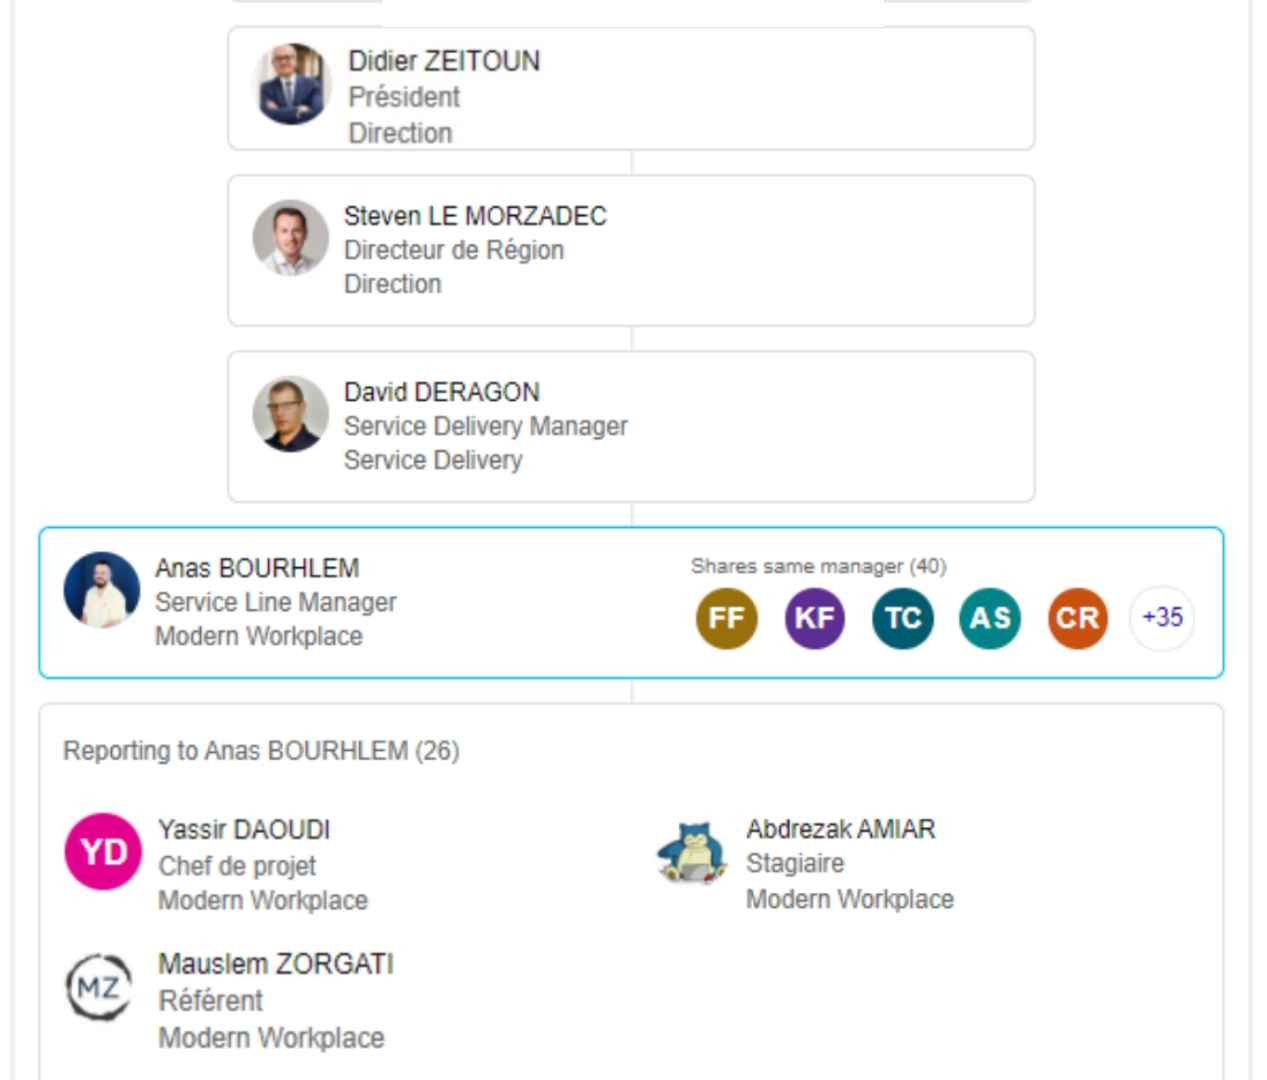
\includegraphics[scale=0.25]{images/StructureOrganisationnelle.jpg}}
		\caption{Structure Organisationnelle EXN}
	\end{center}
\end{figure}

L'équipe comprend d'autres membres qui ne sont pas sous la supervision directe d'Anas Bourhlem.Dans le prochain paragraphe, je présenterai ces membres supplémentaires et expliquerai le rôle de chacun au sein de l'équipe.
\newpage
\subsection{Présentation de l'équipe}


L'équipe Modern Workplace se compose de divers membres ayant des rôles spécifiques et complémentaires pour assurer la réussite de nos projets. Voici une présentation de notre équipe :

\begin{itemize}
    \item[•] \textbf{Steven Le Morzadec} : Directeur de Région, il est la voix décisive pour guider le projet et assure la supervision globale des opérations.
    \item[•] \textbf{Anas Bourhlem} : Service Line Manager (Modern Workplace), il est l’un des spécialistes métier et joue un rôle clé dans la direction et la coordination des activités de l'équipe. Il est aussi mon tuteur de stage.
    \item[•] \textbf{Yassir Daoudi} : Chef de projet, il est le chef d'orchestre assurant la coordination de toutes les étapes du projet et garantissant que les objectifs sont atteints de manière efficace.
    \item[•] \textbf{Marc Kruzik} : Consultant Apps \& Infra \& Data, il aide au niveau technique et assure un rôle de coach pour le développement des compétences techniques.
    \item[•] \textbf{Mauslem Zorgati} : Consultant SharePoint, il apporte son expertise pour les configurations SharePoint spécifiques à notre solution et plus généralement sur Microsoft 365.
    \item[•] \textbf{Pisda Phcar} : Graphiste Designer, il apporte sa créativité et ses compétences en design graphique pour améliorer l'ergonomie de notre projet.
    \item[•] \textbf{Abdrezak Amiar (Auteur)} : Développeur, il est l'artisan du code, responsable de la programmation et du développement des solutions techniques.
\end{itemize}




\section{Définition des objectifs du stage}
\subsection{Description des objectifs globaux du stage}

Le stage a pour objectif principal de développer une interface d'administration pour les scripts d'audits et de gouvernance des systèmes d'information (\textbf{SI}) Microsoft365. Cette interface vise à industrialiser les processus d'audit de tout ou partie d'un SI collaboratif en utilisant des technologies telles que Microsoft .NET, Azure, M365 et PowerShell.

\subsection{Importance et impact attendu sur l’entreprise}

L'importance de ce projet pour l'entreprise réside dans l'amélioration de l'efficacité et de la précision des audits SI. L'interface permettra de centraliser et d'automatiser les audits, réduisant ainsi les erreurs manuelles et augmentant la rapidité des processus. Cela aidera Exakis Nelite à offrir des services de haute qualité à ses clients, renforçant ainsi sa position sur le marché en tant qu'expert en transformation digitale et gouvernance SI.

\newpage

\subsection{Compétences à développer ou acquérir}

Au cours de ce stage, plusieurs compétences clés seront développées ou renforcées :
\begin{itemize}
    \item[•] \textbf{Techniques de développement} : Maîtrise de l'environnement Microsoft et Azure pour le Modern Workplace, utilisation de \textbf{.NET} \textbf{C\#} et \textbf{PowerShell} pour le développement d'applications, et expertise en \textbf{Azure} \textbf{DevOps} et pipelines CI/CD pour le déploiement.
    \item[•] \textbf{Gestion de projets} : Compréhension et application des méthodologies Agile pour planifier et exécuter des projets.
    \item[•] \textbf{Compétences fonctionnelles} : Analyse des besoins utilisateurs, rédaction des User Stories et conception de solutions adaptées.
    \item[•] \textbf{Sécurité informatique} : Connaissance des bonnes pratiques de sécurité et de conformité pour les systèmes Microsoft 365 et Cloud Azure.
\end{itemize}

\subsection{Livrables et indicateurs de réussite}
Les livrables attendus du stage incluent :
\begin{itemize}
    \item[•] \textbf{Interface d'administration} : Une application web fonctionnelle pour la gestion des scripts d'audit.
    \item[•] \textbf{Documentation technique} : Guides et manuels pour l'utilisation et la maintenance de l'interface.
    \item[•] \textbf{Rapports d'audit} : Modèles de rapports automatisés générés par l'interface.
\end{itemize}

Les indicateurs de réussite pour l'entreprise et pour moi sont :
\begin{itemize}
    \item[•] \textbf{Pour l'entreprise} :
    \begin{itemize}
        \item Réduction du temps nécessaire pour réaliser des audits SI.
        \item Augmentation de la précision des audits grâce à l'automatisation.
        \item Satisfaction des clients grâce à une meilleure qualité des rapports d'audit.
    \end{itemize}
    \item[•] \textbf{Pour moi} :
    \begin{itemize}
        \item Acquisition de compétences techniques avancées en développement et sécurité.
        \item Compréhension approfondie des processus de gouvernance SI.
        \item Réussite dans la gestion et la livraison d'un projet complet en suivant les méthodologies Agile.
    \end{itemize}
\end{itemize}

\newpage

\section{Récapitulatif}
\textit{Dans ce chapitre introductif, j'ai présenté l'organisme d'accueil, en commençant par une introduction à l'université, puis à l'entreprise et à l'équipe. J'ai détaillé l'historique, la mission, ainsi que les produits et services principaux de l'entreprise. Ensuite, j'ai décrit la composition et les rôles des membres de l'équipe, ainsi que leurs objectifs et missions. J'ai également examiné la structure organisationnelle pour mettre en lumière la position de l'équipe au sein de l'entreprise. Enfin, j'ai défini les objectifs du stage, en précisant les objectifs globaux, l'importance et l'impact attendu sur l'entreprise, les compétences à développer, ainsi que les livrables et les indicateurs de réussite.}

\textit{Le chapitre suivant abordera le cadrage fonctionnel du projet.}
